\documentclass[a4paper,12pt]{report}

\usepackage{alltt, fancyvrb, url}
\usepackage{graphicx}
\usepackage[utf8]{inputenc}
\usepackage{float}
\usepackage{hyperref}

\usepackage[italian]{babel}

\usepackage[italian]{cleveref}

\usepackage[table]{xcolor}
\usepackage{array}
\usepackage{multirow}
\usepackage{titlesec}

\titleformat{\chapter}[display]
  {\normalfont\bfseries}{}{0pt}{\Huge}


\title{\textbf{Pcd-Assigment02 Report}\\\large Find the Dependencies}
\author{
Bedeschi Federica \\
\textit{0001175655 federica.bedeschi4@studio.unibo.it}\\\\
Pracucci Filippo \\
\textit{0001183555 filippo.pracucci@studio.unibo.it}
}

\date{Anno accademico 2024-2025}



\begin{document}
\maketitle
\newpage

\tableofcontents

% ANALISI
% A brief analysis of the problem, focusing in particular aspects that are relevant from concurrent point of view.
\chapter{Analisi}
\section{Descrizione del problema}
\subsection{Programmazione asincrona}
Il problema richiedeva lo sviluppo di una liberia asincrona \texttt{DependencyAnalyserLib} per effettuare l'analisi delle dipendenze di un progetto Java, tenendo traccia dei tipi (interfacce/classi) e dei package utilizzati da ogni interfaccia/classe/package del progetto. La libreria comprende lo sviluppo di tre metodi asincroni:
\begin{itemize}
    \item \texttt{getClassDependencies(classSrcFile)}: produce come risultato la lista dei tipi usati dalla classe;
    \item \texttt{getPackageDependencies(packageSrcFolder)}: produce come risultato la lista dei tipi usati da tutti i sorgenti del package;
    \item \texttt{getProjectDependencies(projectSrcFolder)}: produce come risultato la lista dei tipi usati da tutti i sorgenti del progetto.
\end{itemize}
Abbiamo deciso di implementare un metodo per escludere alcune dipendenze. Nel nostro caso l'abbiamo utilizzato per escludere le dipendenze del package java.lang, in quanto contiene i tipi standard del linguaggio.
\subsection{Programmazione reattiva}
Il problema richiedeva lo sviluppo di un programma con interfaccia grafica chiamato \texttt{DependencyAnalyser}, usando un approccio basato sulla programmazione reattiva. Questo fornisce la possibilità di analizzare e mostrare dinamicamente/incrementalmente un grafo delle dipendenze trovate nelle interfacce/classi del progetto selezionato dall'utente, raggruppandole per interfaccia/classe e per package.
\section{Visione concorrente}
In entrambi i casi abbiamo adottato il linguaggio Java; per fare il parsing dei sorgenti e generare gli AST abbiamo utilizzato la libreria \href{https://javaparser.org/}{JavaParser}.\\
Per quanto riguarda la programmazione asincrona abbiamo utilizzato il framework \href{https://vertx.io/}{Vert.x}. 
L'implementazione dei tre metodi asincroni produce come valore di ritorno una \texttt{Future} del relativo report delle dipendenze.\\
Per quanto riguarda la programmazione reattiva abbiamo utilizzato il framework \href{https://github.com/ReactiveX/RxJava}{RxJava}, tramite il quale creiamo uno stream delle dipendenze di ogni singolo sorgente, reagendo alla produzione di ogni elemento con l'aggiornamento della GUI, così da ottenere un comportamento incrementale.

% DESIGN E ARCHITETTURA
% A description of the adopted design, the strategy and architecture.
% A description of the behaviour of the system using one or multiple Petri Nets, choosing the propor level of abstraction.
\chapter{Design e architettura}
\section{Programmazione asincrona}
Il metodo \texttt{getClassDependencies} ha il compito di analizzare un singolo sorgente e trovarne le dipendenze, mentre gli altri due si occupano di capire la struttura del file system partendo dalla directory sorgente per poi richiamarsi a cascata fino ad arrivare a \texttt{getClassDependencies} in modo da ottenere le dipendenze dei singoli sorgenti.
Ogni metodo produce una diversa tipologia di report delle dipendenze, anch'essi composti nella modalità sopracitata.
Abbiamo inserito una classe di test per mostrare un comportamento tipico di utilizzo della libreria.
\subsection{Rete di Petri}
La rete di Petri in \Cref{fig:petri-net-async} descrive il comportamento del sistema, mostrando la composizione dei metodi come descritto sopra. Il sistema parte con un singolo token ad effettuare la transizione \texttt{getProjectDependencies}, per poi generare tanti token quanti sono i package. Successivamente viene eseguita la transizione \texttt{getPackageDependencies}, generando tanti token quante sono le classi/interfacce, per poi eseguire la transizione \texttt{getClassDependencies}.
\begin{figure}[H]
    \centering
    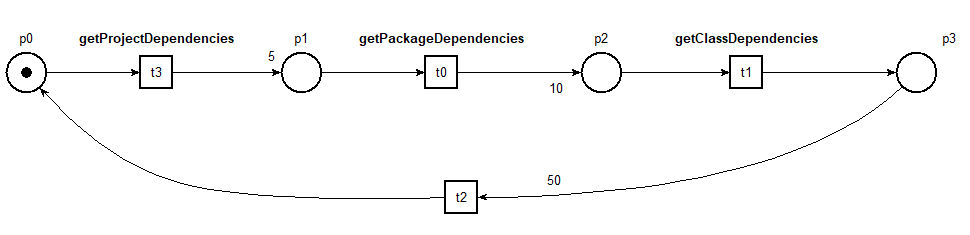
\includegraphics[width=\linewidth]{figures/async.png}
    \caption{\centering Rete di Petri - programmazione asincrona \newline \textit{Il 5 presente in figura rappresenta in realtà il numero di package del progetto, mentre il 10 rappresenta un valore simbolico del numero di classi di ogni package.}}
    \label{fig:petri-net-async}
\end{figure}
\section{Programmazione reattiva}
Abbiamo optato per un'architettura che seguisse il pattern \textit{MVC}, come mostrato in \Cref{fig:class-diagram-reactive}, quindi con un \textit{Controller} che si occupasse di mettere in comunicazione il \textit{Model} con la \textit{View}.
Il Controller ha il compito di ottenere dal \texttt{DependencyAnalyser} l'\texttt{Observable} dello stream composto dai report delle dipendenze di ogni classe/interfaccia, sul quale effettua la \texttt{subscribe} per aggiornare la GUI incrementalmente.
La visualizzazione delle dipendenze avviene utilizzando un albero in cui le foglie sono le dipendenze raggruppate per sorgente e per package.
\begin{figure}[H]
    \centering
    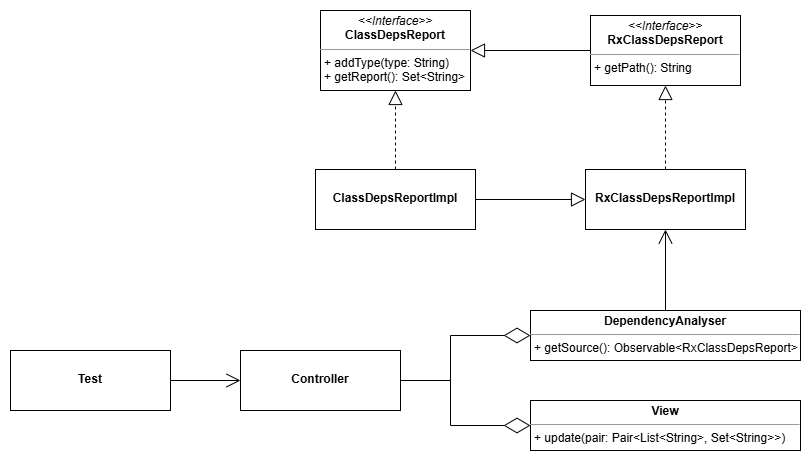
\includegraphics[width=\linewidth]{figures/class_diagram_reactive.png}
    \caption{\centering Diagramma delle classi - programmazione reattiva}
    \label{fig:class-diagram-reactive}
\end{figure}
\subsection{Rete di Petri}
La rete di Petri in \Cref{fig:petri-net-reactive} descrive il comportamento del sistema, mostrando la produzione continua di token tramite la transizione \texttt{getClassDependencies}, che rappresentano i report prodotti. In seguito alla produzione di un report viene eseguita la transizione \texttt{UpdateGUI}. Abbiamo inserito la transizione \textit{t2} per simulare la terminazione dei file sorgenti, che conclude l'esecuzione.
\begin{figure}[H]
    \centering
    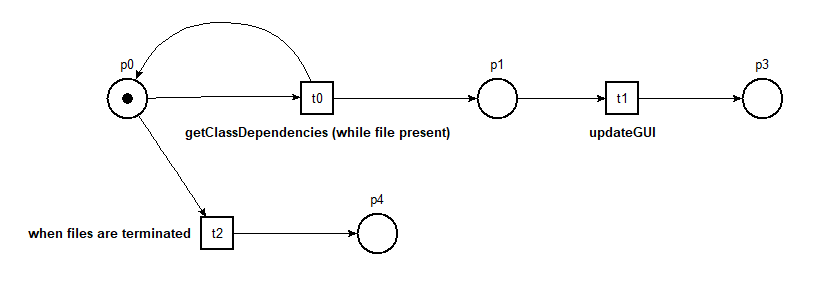
\includegraphics[width=\linewidth]{figures/reactive.png}
    \caption{\centering Rete di Petri - programmazione reattiva}
    \label{fig:petri-net-reactive}
\end{figure}

%CONCLUSIONI
\chapter{Conclusioni}
La libreria realizzata con un approccio asincrono ci ha permesso di sfruttare le caratteristiche del paradigma, cioè consentendo la continuazione dell'esecuzione senza dover rimanere bloccati in attesa del risultato.
Inoltre, trattandosi di una libreria, è possibile utilizzarla per diverse applicazioni, sfruttando i metodi utili nel caso specifico; nel nostro caso è stato realizzato un semplice test per mostrare il suo funzionamento. \\
Per quanto riguarda la programmazione reattiva abbiamo potuto notare come quest'ultima sia particolarmente adatta in un contesto incrementale, quindi per esempio nel nostro caso è perfetta per ottenere un aggiornamento dinamico dell'interfaccia grafica, grazie alla flessibilità offerta dall'utilizzo degli stream.

\end{document}
